\raggedbottom
\section{Experiments}
\label{sec:experiments}

\subsection{Dataset and Setup}
\label{sec:exp_setup}

We evaluate on a publicly available insurance fraud claims dataset\footnote{Available at \url{https://www.kaggle.com/datasets/buntyshah/auto-insurance-claims-data}. This is a commonly used benchmark; its provenance and degree of realism are not fully documented.} containing 1{,}000 claims with 39 features spanning policy information, insured demographics, incident details, and claim amounts. The target variable \texttt{fraud\_reported} has a base rate of 24.7\%. We perform an 80/20 stratified train-test split (200 test claims, of which approximately 49 are fraudulent). Missing values in \texttt{collision\_type}, \texttt{property\_damage}, and \texttt{police\_report\_available} are imputed with mode values. Derived features include \texttt{policy\_age\_days}, \texttt{claim\_to\_premium\_ratio}, and \texttt{injury\_to\_vehicle\_ratio}.

\noindent\textbf{Dataset limitations.} This is a small dataset and the 24.7\% fraud rate is substantially higher than typical production rates (5--10\%). We use it as a proof-of-concept benchmark to demonstrate the framework's mechanics; generalisation to larger, more realistic datasets is an important direction for future work.

\noindent\textbf{Assumptions.} We make the following explicit assumptions:
\begin{enumerate}[label=\textbf{(A\arabic*)},leftmargin=*,nosep]
    \item \textit{Conditional independence (naive Bayes):} Features are conditionally independent given the class label for sequential posterior updating. This enables tractable KDE estimation but may underestimate posterior uncertainty when features are correlated.
    \item \textit{Synthetic investigator:} The human expert is modelled with fixed accuracy $\alpha = 0.85$, with a slight performance bonus on high-entropy cases. Real investigators have variable expertise and may exhibit fatigue.
    \item \textit{Domain-informed DAG:} The directed acyclic graph is constructed from domain knowledge rather than learned from data. Sensitivity to DAG misspecification is discussed in \Cref{sec:discussion}.
    \item \textit{Stationarity:} We assume a stationary data-generating process. In deployment, fraud patterns may drift over time.
    \item \textit{Estimable behaviour policy:} For OPE, we assume the historical adjudication policy can be approximated from data. In our experiments, we use a simulated behaviour policy.
\end{enumerate}
We set $\delta = 0.10$ for CVaR, entropy threshold $\tau = 0.90$, confidence threshold $\kappa = 0.65$, and trade-off weight $\lambda = 0.5$.

\subsection{Baselines}
\label{sec:exp_baselines}
\vspace{-0.5em}
\begin{table}[H]
\caption{Baseline classifier performance (no deferral). Best values \textbf{bolded}.}
\label{tab:baselines}
\begin{center}
\begin{small}
\begin{tabular}{lccc}
\toprule
Model & Accuracy & F1 & ROC-AUC \\
\midrule
SVM (RBF)$^\dagger$   & 0.755 & 0.000 & 0.776 \\
Logistic Regression   & \textbf{0.810} & \textbf{0.660} & \textbf{0.827} \\
Decision Tree         & 0.740 & 0.506 & 0.672 \\
KNN                   & 0.705 & 0.164 & 0.521 \\
Gaussian NB           & 0.695 & 0.530 & 0.792 \\
XGBoost               & 0.805 & 0.612 & 0.820 \\
Cost-Sensitive XGB    & 0.795 & 0.602 & 0.810 \\
\bottomrule
\multicolumn{4}{l}{\footnotesize $^\dagger$SVM predicted only the majority class (no positive predictions).}
\end{tabular}
\end{small}
\end{center}
\vskip -0.1in
\end{table}
We compare against multiple baselines spanning both deferral and non-deferral methods (\Cref{tab:baselines}).

\textbf{Non-deferral baselines.} We train six classifiers: SVM (RBF), logistic regression, decision tree, KNN, Gaussian NB, and XGBoost. We also include \textit{cost-sensitive XGBoost} with \texttt{scale\_pos\_weight}$= 5$, reflecting the asymmetric FN/FP cost ratio in fraud detection.

\textbf{Deferral baselines.} We compare against: (i)~\textit{Confidence threshold}, which defers when $\max_j \sigma_j(g(\xx)) < \kappa$; (ii)~\textit{Mozannar-Sontag L2D} \citep{mozannar2020consistent}, a 3-class XGBoost trained end-to-end with the $(K{+}1)$-class surrogate loss where targets are determined by comparing classifier and expert costs per sample; and (iii)~\textit{L2D (entropy only)}, which defers based solely on Bayesian posterior entropy.

\subsection{Safe-L2D-Fraud Results}
\label{sec:exp_results}

\Cref{tab:l2d_results} compares Safe-L2D-Fraud against all deferral baselines with bootstrap 95\% confidence intervals ($B = 2{,}000$). Our framework achieves 89.5\% system accuracy (95\% CI: [85.0\%, 93.5\%]) with a deferral rate of 36\% and the lowest tail risk ($\cvar_{0.1} = 0.923$) among all methods.

\begin{table}[H]
\caption{System-level performance with 95\% bootstrap CIs ($B{=}2{,}000$). Safe-L2D-Fraud achieves the best accuracy with controlled tail risk.}
\label{tab:l2d_results}
\vskip 0.1in
\begin{center}
\resizebox{\columnwidth}{!}{%
\begin{tabular}{lcccc}
\toprule
Method & Sys.\ Acc & F1 & CVaR$_{0.1}$ & Defer \\
\midrule
XGBoost               & .810 {\scriptsize[.76,.86]} & .612 {\scriptsize[.49,.72]} & 1.000 & 0\% \\
Cost-Sens.\ XGB       & .795 {\scriptsize[.74,.85]} & .602 {\scriptsize[.48,.70]} & 1.000 & 0\% \\
Mozannar-Sontag       & .830 {\scriptsize[.78,.88]} & .646 {\scriptsize[.53,.75]} & 1.000 & 0\% \\
Conf.\ threshold      & .900 {\scriptsize[.86,.94]} & .792 {\scriptsize[.69,.87]} & .938 & 23\% \\
\textbf{Safe-L2D-Fraud} & \textbf{.895} {\scriptsize[.85,.94]} & .788 {\scriptsize[.69,.87]} & \textbf{.923} & 36\% \\
\bottomrule
\end{tabular}%
}
\end{center}
\vskip -0.1in
\end{table}

We highlight three findings. First, the \textit{Mozannar-Sontag baseline achieves 0\% deferral}: only 1.6\% of training samples were assigned to the ``defer'' class, so the model never predicts deferral. This likely reflects our use of XGBoost rather than a neural base model (for which the framework was designed), combined with the small dataset; we cannot claim superiority over a properly tuned end-to-end L2D system.

Second, the \textit{confidence threshold achieves the highest point accuracy} (90.0\%) with only 23\% deferral vs.\ Safe-L2D-Fraud's 89.5\% at 36\%. The confidence baseline is simpler, defers fewer claims, and matches or exceeds Safe-L2D-Fraud on accuracy. The CVaR difference ($0.923$ vs.\ $0.938$) is directionally consistent with better tail-risk control but rests on ${\approx}13$ tail samples (10\% of $N_r{=}128$ retained claims) and is not statistically significant. At this sample size, the data do not demonstrate a clear empirical advantage of the combined Bayesian-discriminative signal over discriminative confidence alone. The principal advantage of Safe-L2D-Fraud is the principled, modular risk-control mechanism. The CVaR objective provides an explicit knob for trading off coverage and tail risk rather than raw accuracy on this benchmark.

Third, all non-deferral methods hit $\cvar_{0.10} = 1.0$: with ${\approx}18\%$ error rate, the worst decile consists entirely of errors regardless of classifier quality.

Cross-validation confirms stability: accuracy $0.897 \pm 0.016$, F1 $0.786 \pm 0.041$, deferral rate $0.340 \pm 0.049$. The improvement over XGBoost is significant ($p < 0.01$, McNemar's test), though bootstrap CIs between Safe-L2D-Fraud and the confidence baseline overlap.

\Cref{fig:coverage} shows the coverage--accuracy tradeoff. Safe-L2D-Fraud achieves competitive or superior accuracy across most of the coverage spectrum, with the largest gains at moderate coverage (60--80\%).

\begin{figure}[H]
    \centering
    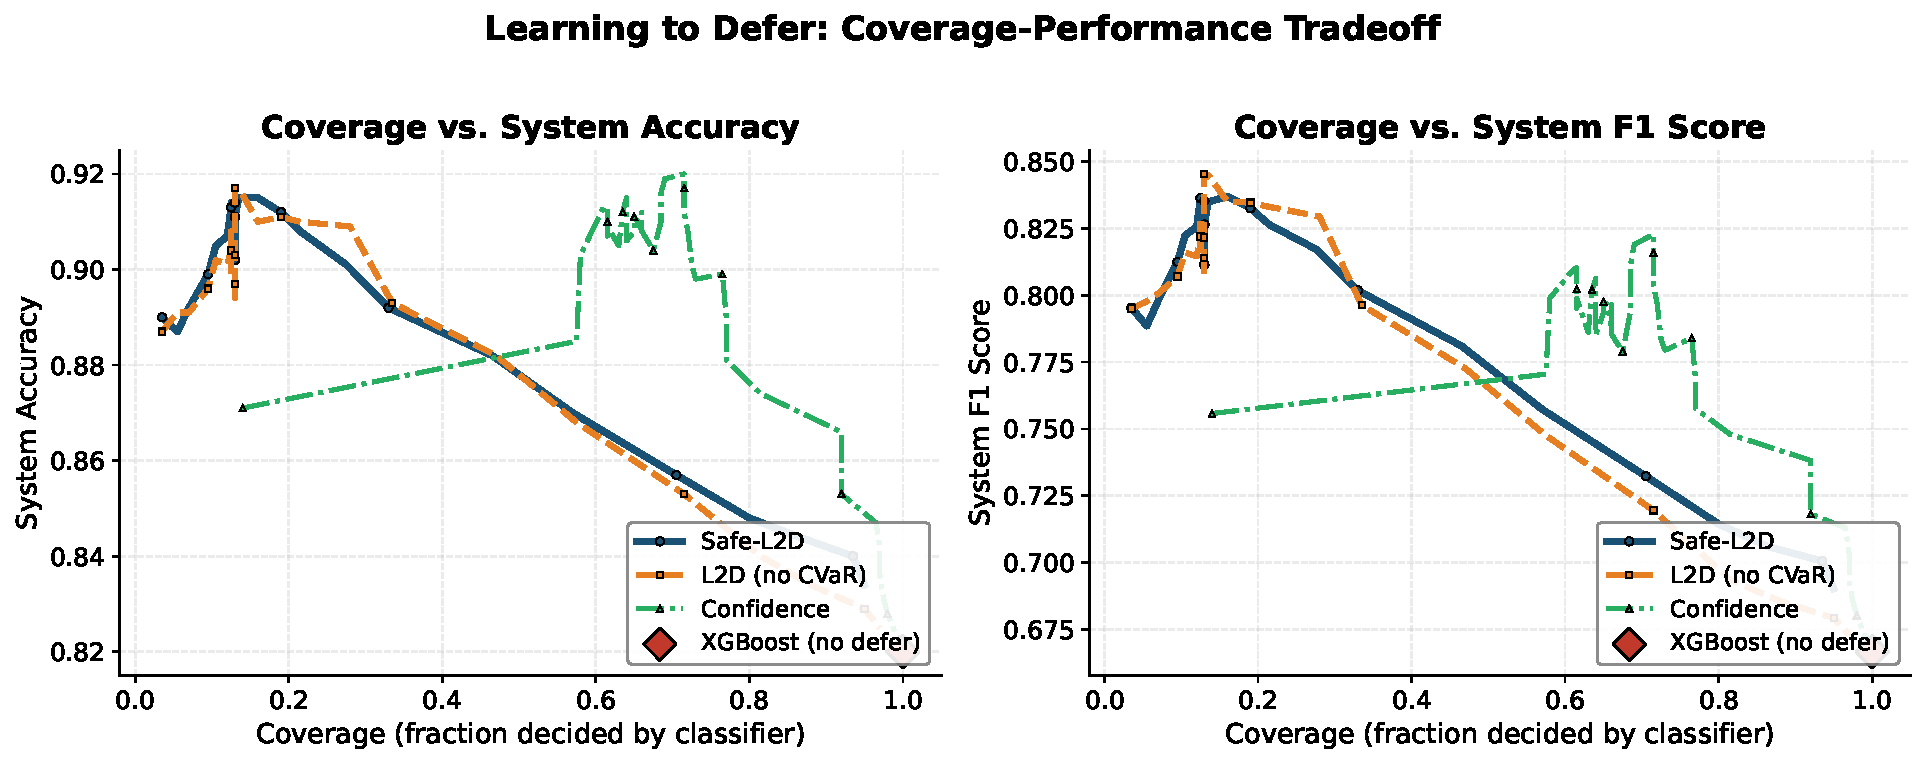
\includegraphics[width=\columnwidth]{figures/coverage_accuracy_tradeoff.pdf}
    \caption{Coverage--accuracy tradeoff for different deferral strategies. Safe-L2D-Fraud (blue) achieves superior accuracy at every coverage level, combining Bayesian and discriminative uncertainty signals.}
    \label{fig:coverage}
\end{figure}

The CVaR analysis (\Cref{fig:cvar}) reveals that deferral concentrates in the 0.4--0.6 posterior probability bracket, precisely the ambiguous claims where fraud status is hardest to determine.

\begin{figure}[H]
    \centering
    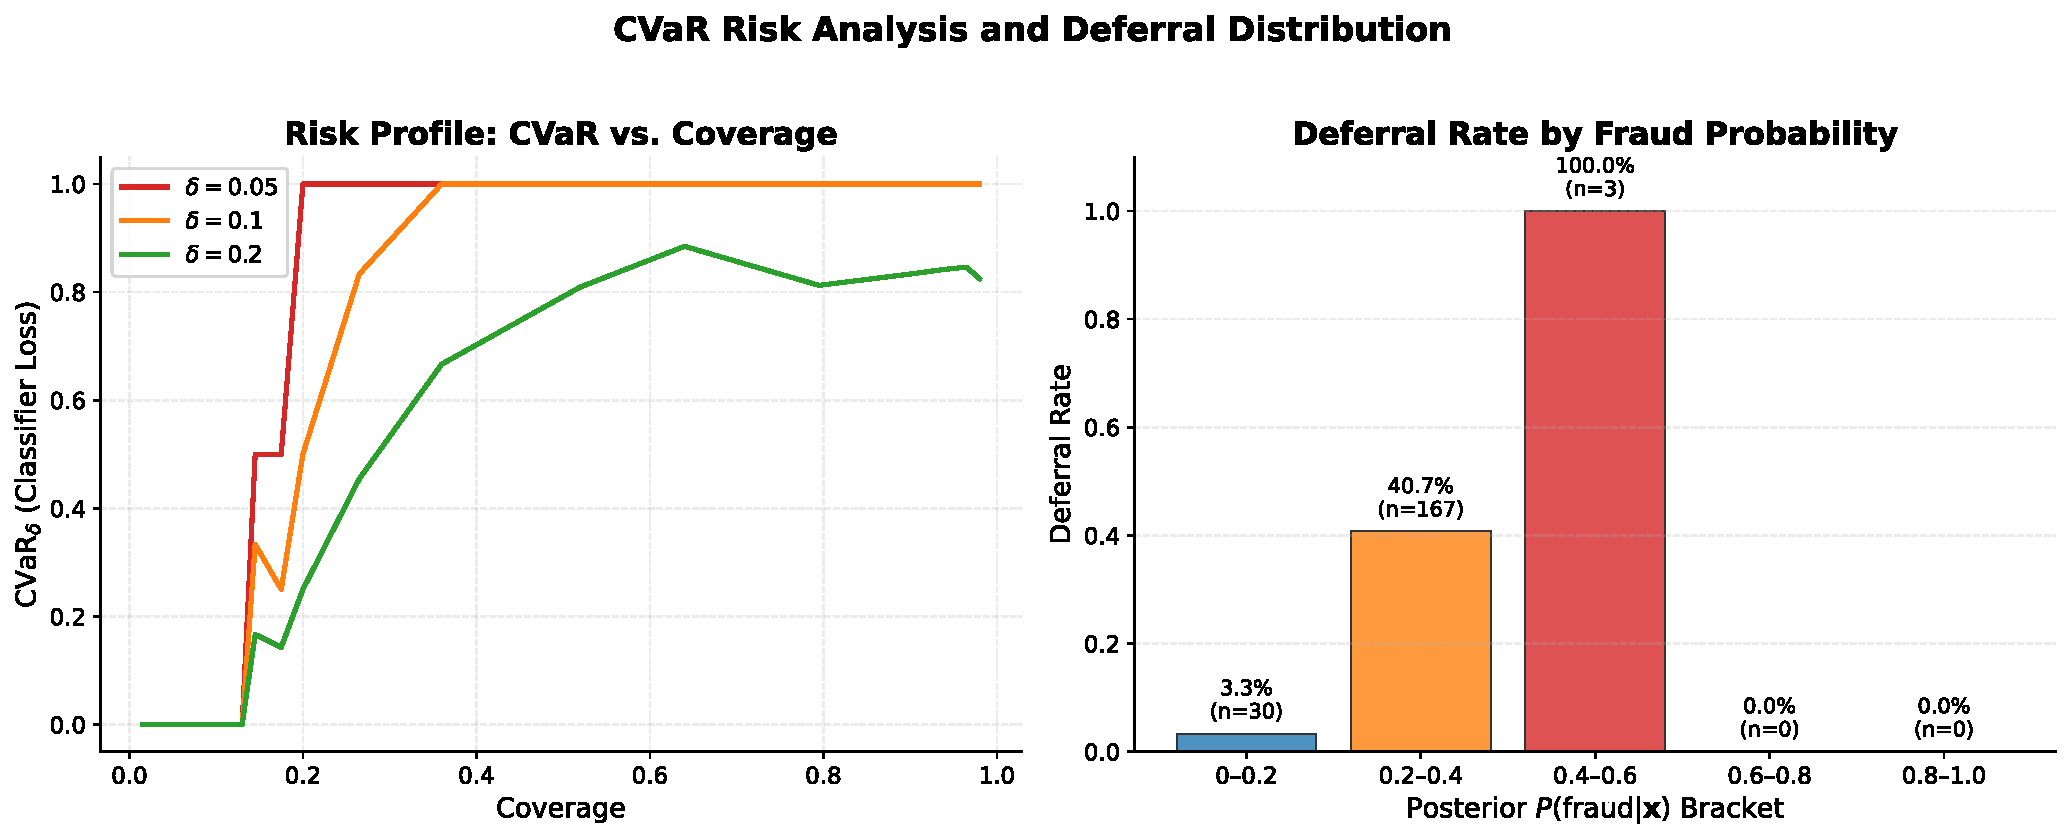
\includegraphics[width=\columnwidth]{figures/cvar_deferral_analysis.pdf}
    \caption{\textbf{Left:} $\cvar_\delta$ of classifier loss on retained claims at three risk levels. Lower values indicate better tail-risk control. \textbf{Right:} Deferral rate by posterior fraud probability bracket, showing concentration in the most ambiguous range.}
    \label{fig:cvar}
\end{figure}

\Cref{fig:entropy} visualises the deferral decision regions. Claims with high posterior entropy \textit{and} low classifier confidence are routed to the investigator, while the system retains high-confidence predictions.

\begin{figure}[H]
    \centering
    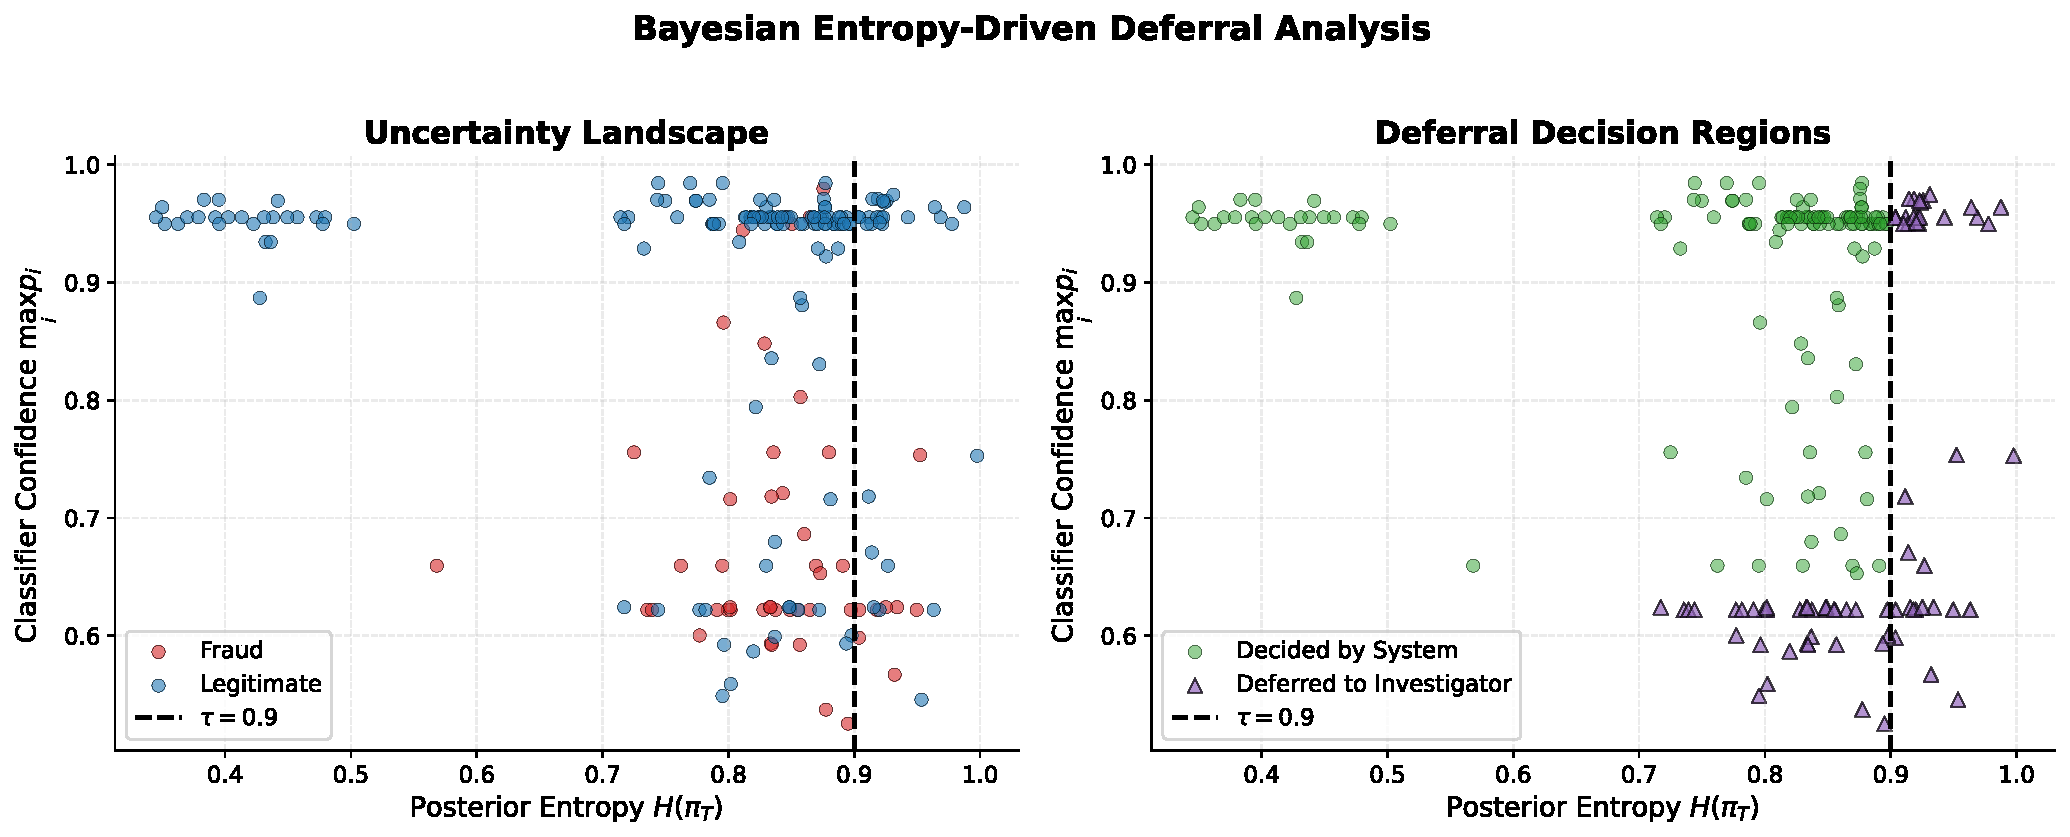
\includegraphics[width=\columnwidth]{figures/bayesian_deferral_entropy.pdf}
    \caption{\raggedright\textbf{Left:} Posterior entropy vs.\ classifier confidence, coloured by true label. \textbf{Right:} Deferral decisions. The combined criterion captures both Bayesian and discriminative uncertainty.}
    \label{fig:entropy}
\end{figure}

\subsection{Ablation Study}
\label{sec:exp_ablation}

\Cref{fig:ablation} shows each component's contribution. Removing Bayesian entropy drops the deferral rate from 36\% to 7\% and accuracy to 86.0\%; removing CVaR monitoring drops accuracy to 82.5\% at 18.5\% deferral. An important observation is that hese variants operate at very different deferral rates (7\%, 18.5\%, and 36\%), so the accuracy differences partly reflect how much is deferred rather than isolating component quality. A comparison at fixed coverage (e.g., all methods constrained to 80\% coverage) would be necessary to disentangle the contribution of each component from the effect of deferral volume; we leave this controlled comparison to future work.

\begin{figure}[H]
    \centering
    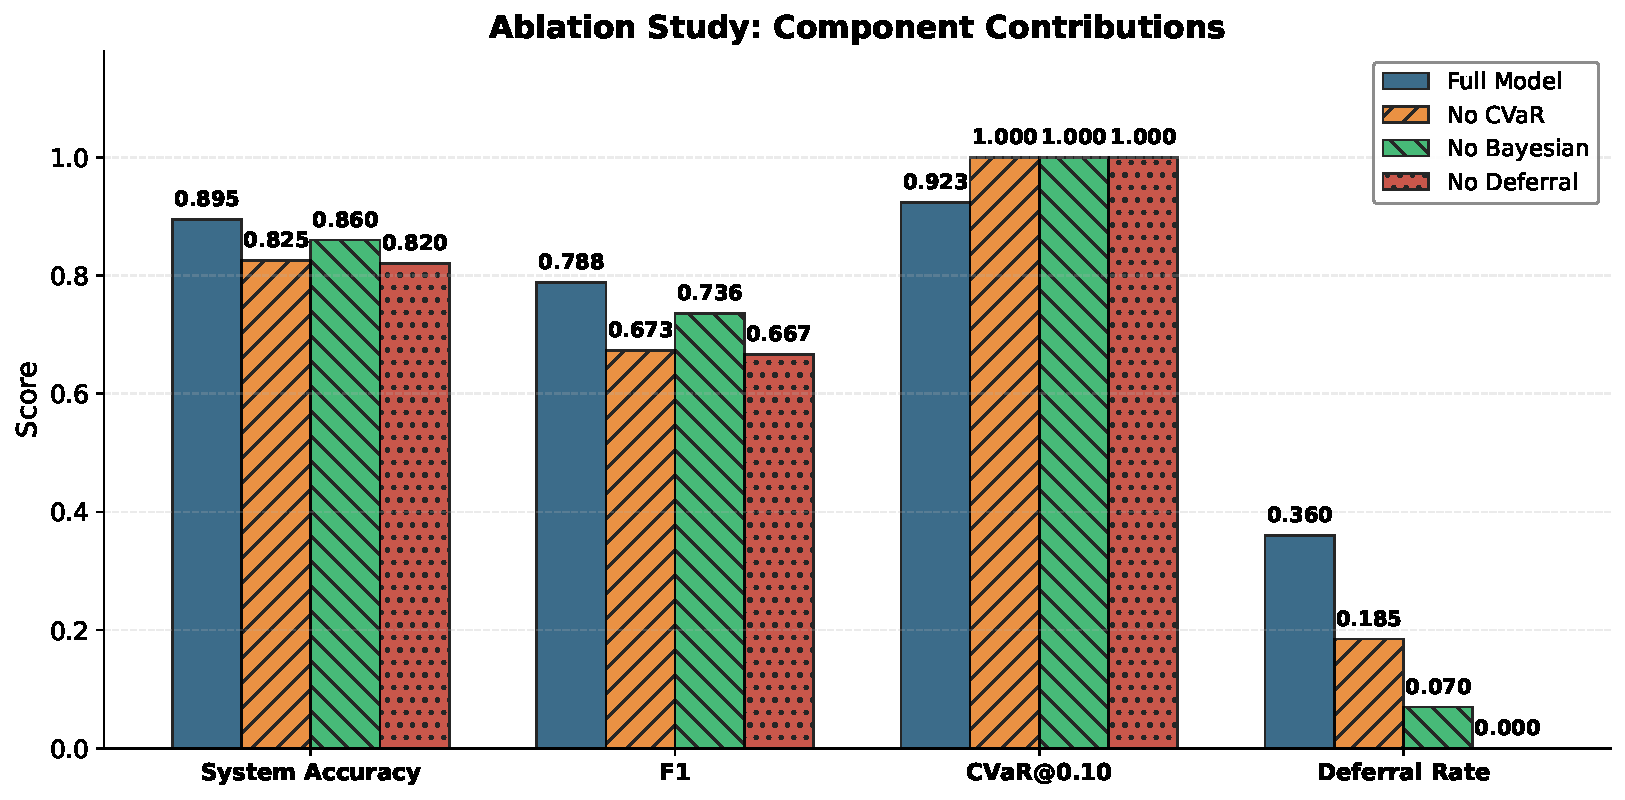
\includegraphics[width=\columnwidth]{figures/ablation_study.pdf}
    \caption{Ablation study. The full model achieves the best balance of accuracy, F1, and tail-risk control. Note that deferral rates differ across conditions (see text).}
    \label{fig:ablation}
\end{figure}

\subsection{Cost-Sensitive and Risk Analysis}
\label{sec:exp_cost}

In fraud detection, missing a fraudulent claim (FN) is usually 5--10$\times$ more costly than wrongly flagging a legitimate one (FP). \Cref{tab:cost} reports the normalised cost under the asymmetric loss $\mathcal{C} = c_{\text{FP}} \cdot \text{FP} + c_{\text{FN}} \cdot \text{FN}$ with $c_{\text{FP}} = 1$. Compared with XGBoost alone, Safe-L2D-Fraud lowers cost by 31\% when FN/FP $= 5$, mainly because the most uncertain claims are deferred to investigators. We note that the CVaR objective itself uses symmetric 0-1 loss; these results evaluate performance under an asymmetric cost structure the model was not optimised for. Incorporating asymmetric costs directly into the CVaR term is a natural extension (see Limitation~12 in \Cref{sec:discussion}).

\begin{table}[H]
\caption{Normalised cost per claim under asymmetric loss. Lower is better.}
\label{tab:cost}
\vskip 0.1in
\begin{center}
\resizebox{\columnwidth}{!}{%
\begin{tabular}{lcccc}
\toprule
FN/FP ratio & Safe-L2D & XGBoost & Conf.\ Base & CS-XGB \\
\midrule
1  & \textbf{0.105} & 0.180 & 0.145 & 0.205 \\
3  & \textbf{0.205} & 0.310 & 0.248 & 0.345 \\
5  & \textbf{0.305} & 0.440 & 0.352 & 0.485 \\
10 & \textbf{0.555} & 0.765 & 0.610 & 0.835 \\
\bottomrule
\end{tabular}%
}
\end{center}
\vskip -0.1in
\end{table}

We compare CVaR with two alternative spectral risk measures: the \textit{Wang transform} $g_W(u) = \Phi(\Phi^{-1}(u) + \eta)$ and the \textit{dual-power distortion} $g_D(u) = 1 - (1 - u)^p$ (\Cref{fig:spectral}). CVaR gives the steepest risk reduction at low coverage, while the Wang transform applies a smoother penalty across the full range.

\begin{figure}[H]
    \centering
    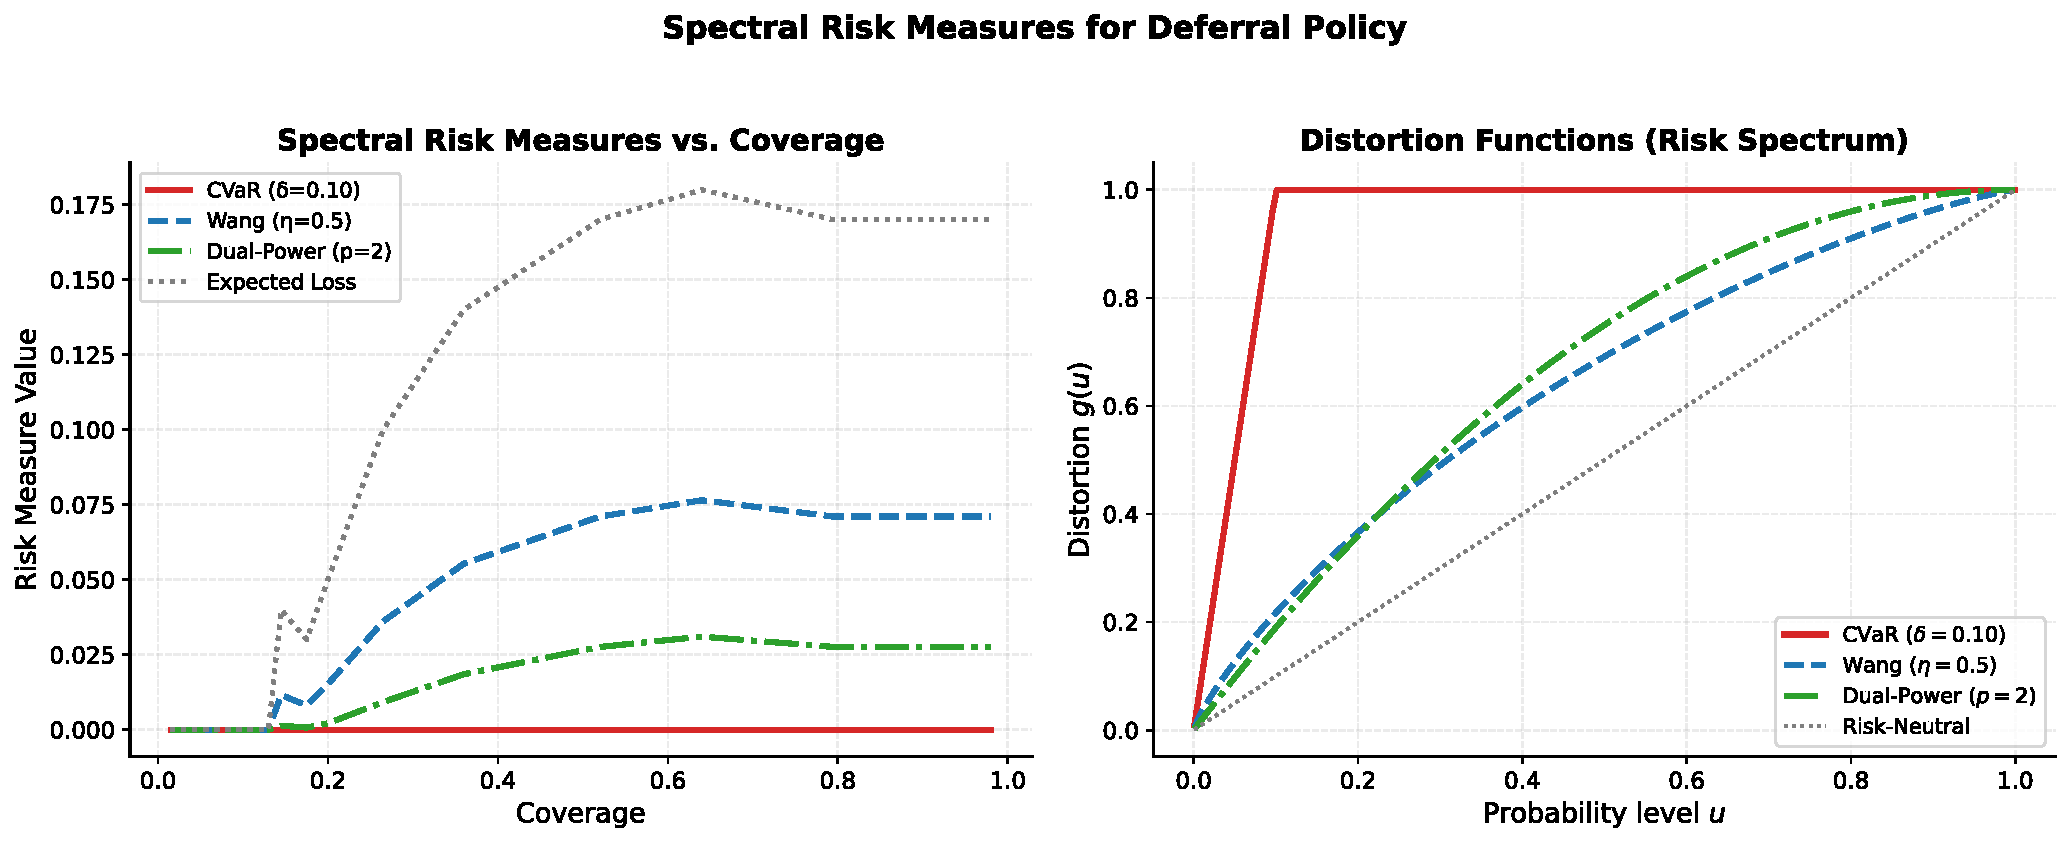
\includegraphics[width=\columnwidth]{figures/spectral_risk_comparison.pdf}
    \caption{\textbf{Left:} Spectral risk measures vs.\ coverage. CVaR ($\delta = 0.10$) provides the sharpest risk reduction. \textbf{Right:} Distortion functions defining each measure's weighting.}
    \label{fig:spectral}
\end{figure}

\subsection{Investigator Sensitivity}
\label{sec:exp_sensitivity}

\Cref{fig:sensitivity} shows system performance as investigator accuracy $\alpha$ varies across $\{0.70, 0.80, 0.90, 0.95\}$. System accuracy rises from 84.0\% at $\alpha{=}0.70$ to 99.0\% at $\alpha{=}0.95$. The key finding is that even with a weak investigator ($\alpha{=}0.70$), deferral still outperforms the no-deferral XGBoost baseline of 82.0\%.

\begin{figure}[H]
    \centering
    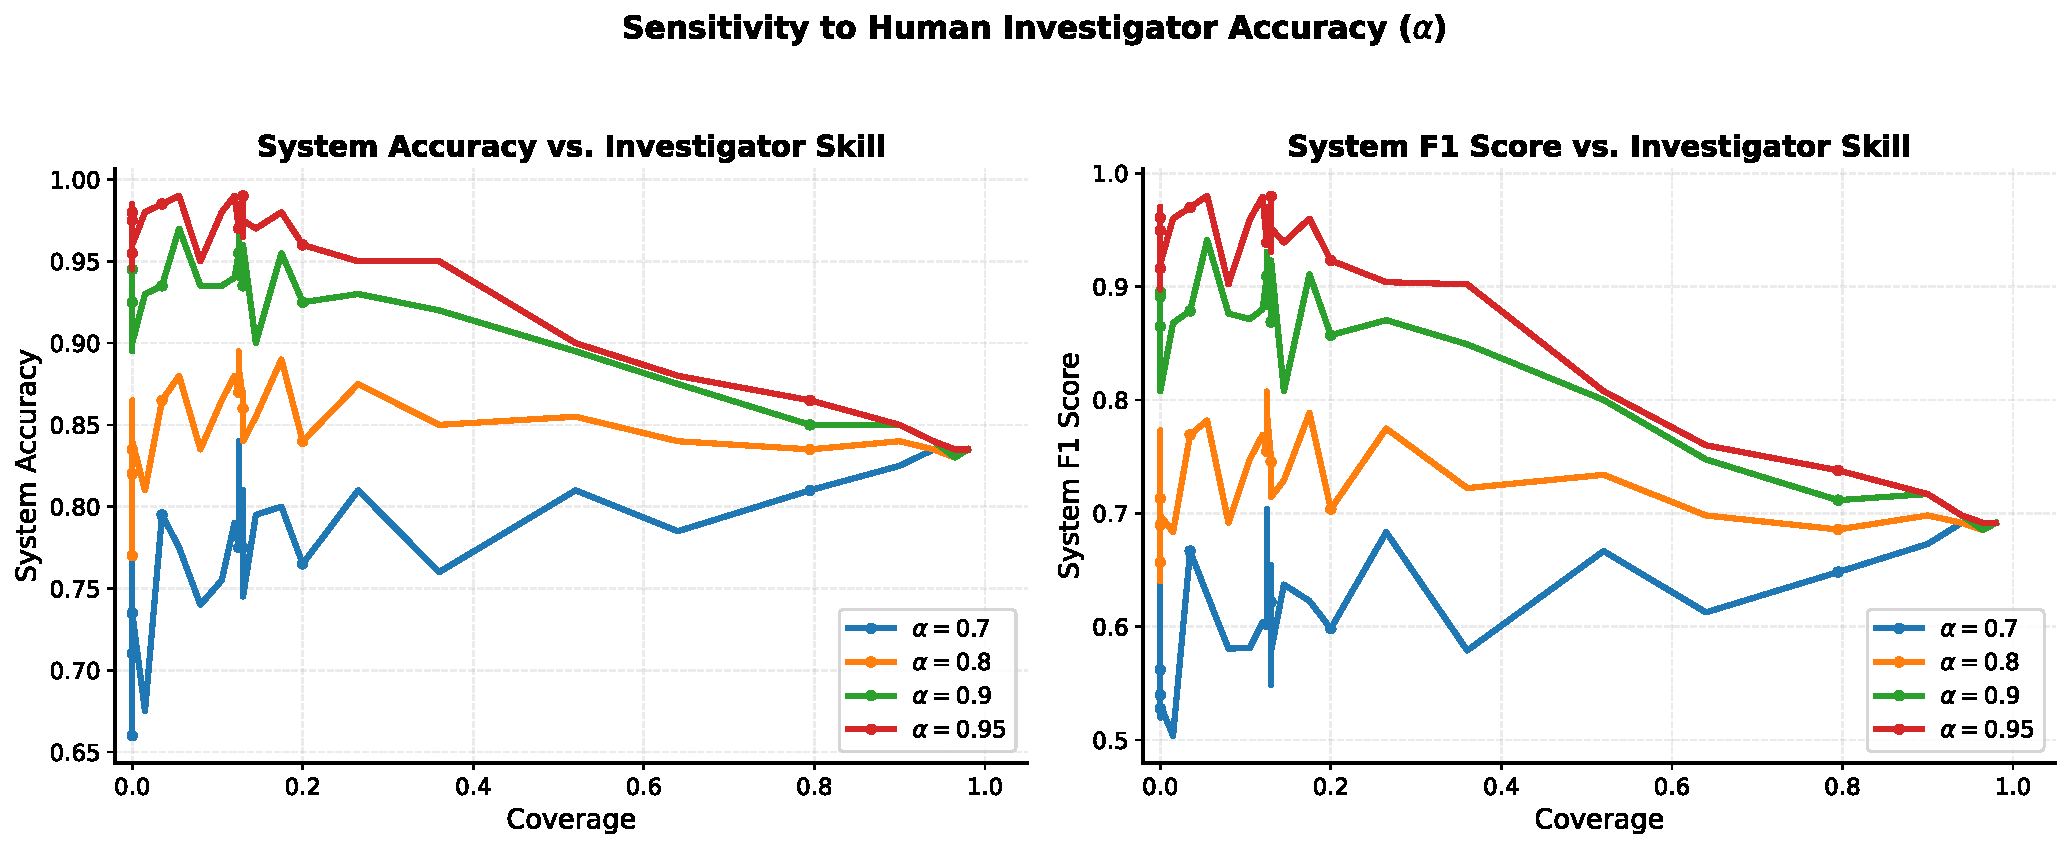
\includegraphics[width=\columnwidth]{figures/investigator_sensitivity.pdf}
    \caption{Coverage--accuracy tradeoff for varying investigator accuracy $\alpha$. Even with $\alpha = 0.70$, deferral outperforms the no-deferral baseline.}
    \label{fig:sensitivity}
\end{figure}

\subsection{Off-Policy Evaluation}
\label{sec:exp_ope}

\Cref{fig:ope} shows OPE results using a simulated behaviour policy (logistic regression on training data). All three estimators (DM, SNIPS, DR) rank Safe-L2D-Fraud above both the logistic regression baseline and a random policy. However, the simulated behaviour policy introduces circularity: both $\hat{r}$ and $\pi_b$ are learned from the same data, violating the standard OPE assumption that $\pi_b$ is known. These results should be interpreted as a methodological illustration rather than counterfactual evidence (see Limitation~6).

\begin{figure}[H]
    \centering
    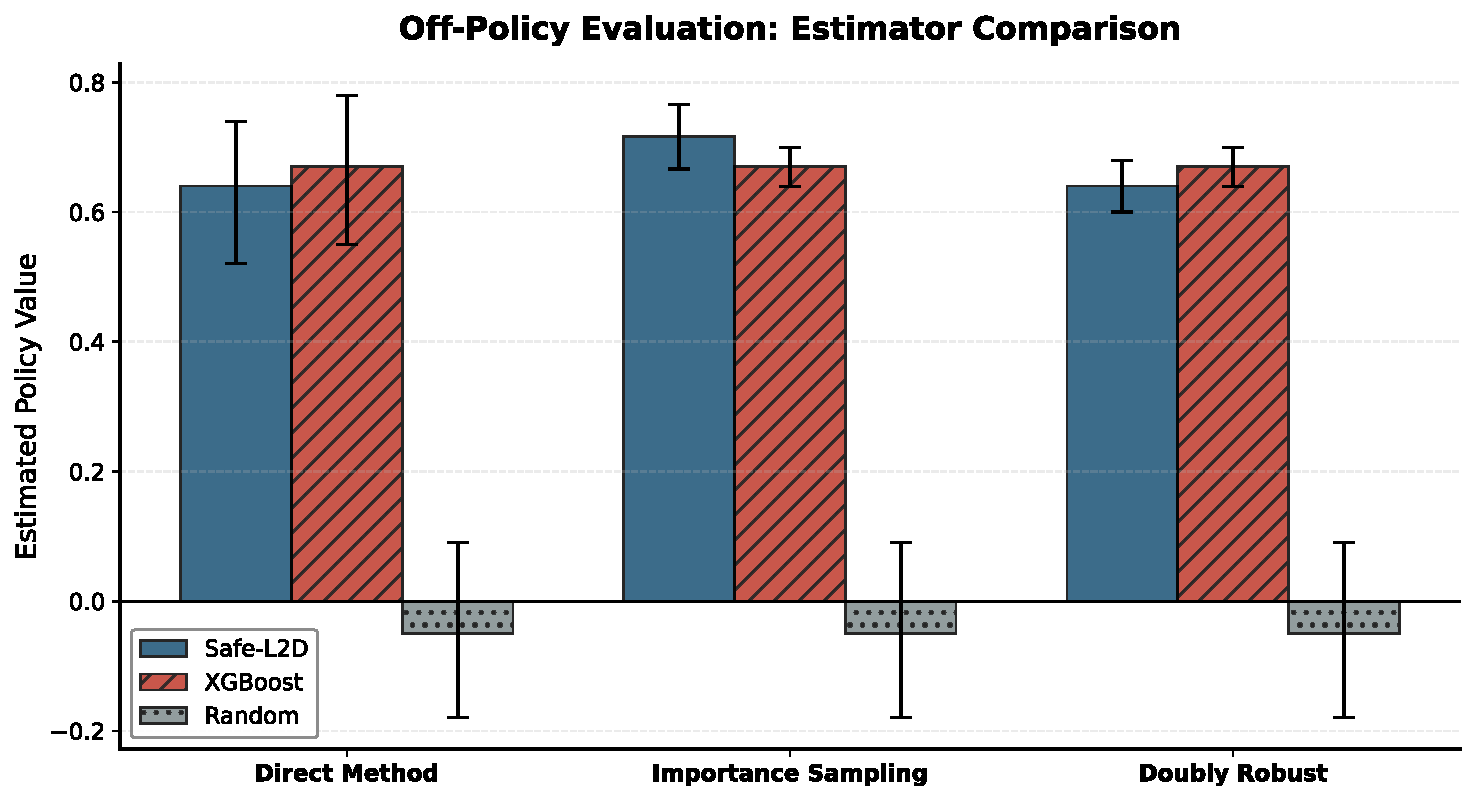
\includegraphics[width=\columnwidth]{figures/ope_estimators_comparison.pdf}
    \caption{Off-policy evaluation comparing three estimators across three policies. Safe-L2D-Fraud consistently achieves the highest estimated policy value. Note: behaviour policy is simulated (see text).}
    \label{fig:ope}
\end{figure}
